\section{Context} \label{sec:intro-context}
While Artificial Intelligence (AI) - as a field - has existed for nearly seventy years \citep{moor2006dartmouth}, the concept of artificial intelligence dates back to at least Ancient Greece.  
In ancient times, artificial intelligence embodied in the dream of mechanical men was part of the domain of myth; in the twentieth century, of that of science.  
During this last decade, Artificial Intelligence is not anymore a part of a single specific domain, as it has materialised out of Man's imagination, broken out of laboratories and has been given lease to act in the world at large.

Artificial Intelligence and specifically Machine Learning, the branch of AI that specialises in creating computer systems able to learn their programming from real-world examples instead of having to be explicitly coded by a human, have in the last two decades seen incredible success\footnote{See \citet{shalev2014understanding} for an introduction to Machine Learning and Figure \ref{fig:ai-overview} to get an overview of the field of AI}.
No sector of our economy has been left untouched by the recent and rapid rise of machine learning that has been enabled by the rediscovery of neural networks, the availability of Big Data and increased availability of parallel computing power\footnote{A compelling talk, explaining the recent rise of ML, by AI pioneer Geoff Hinton can be found at \citet{hintonmachinelearning}}.
Fields as diverse and as critical as are government, healthcare, finance and bioinformatics have been revolutionised and the possibility has been set for new ones - such as self-driving vehicles - to be born\footnote{For an overview of the impacts of AI on current society and labour market see \citet{schwab2017fourth}}.
The ever increasing reliance of our society on ever more complex machine learning-driven algorithms can only make us worry ever more about the ethical problems posed by such a situation.  
Our society has only very recently been confronted with the dilemma of assigning blame when a driverless car causes the death of a person\footnote{See \citet{uberkillspedestrian}}, but this moral issue is only the tip of the iceberg, even when focusing only on the automotive industry.  
As more and more decisions are made in an automated way, with many of them significantly impacting both individuals and society at large, it comes natural to stop and wonder what are the characteristics we would want the systems tasked with making these decisions to possess.  

 \begin{figure}[htbp]
\centerline{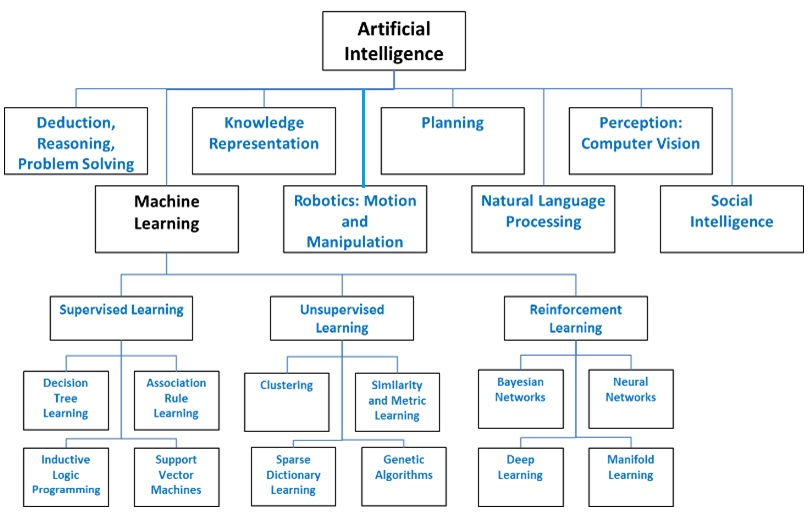
\includegraphics[width=0.7\textwidth]{introduction/images/ai-overview}}
\caption{Dendrogram showing an overview of the field of AI with the position of ML emphasised [source unknown]}
\label{fig:ai-overview}
\end{figure}

\textit{Explainable AI} (xAI) is the sub-field of Artificial Intelligence that ideally should rest at the intersection between Computer Science, Social Sciences and Philosophy and whose aim should be to define the desiderata of artificially intelligent systems and to develop methods to achieve them.
For example, how should a self-driving car behave when confronted with a real-world analogous of the classic Trolley Problem - a situation where each course of action is liable to cause harm?  
On what basis should a person be denied a mortgage, access to university or a job interview?  How can we be sure that there is no bias in the system?  How do we even define if the system is behaving morally?  Would it currently be feasible for a person that feels they have been harmed by such a decision to appeal it?\footnote{For an overview of AI ethics see \citet{Bostrom2011}}
The main idea to achieve these goals is for the systems in question to be somehow made \textit{explainable}. 
The problems start at the very first step, as within the xAI community, as noted by \citet{Doran2018}, there is currently no unanimously agreed upon definition of the definition of \textit{explainability} and consequently of the best way to achieve it in real systems.
The review carried out in Section \ref{sec:explainability} highlights one of the fundamental problems of the field of xAI: that all researchers within the community claim their methods to be \enquote{explainable}, but very few justify this with reasons grounded in the real world (as best noted by the popular paper by \citet{Lipton2016}).

To solve this conundrum various authors have tried to define taxonomies into which classify systems, based on their characteristics and how these relate to its perceived explainability.
One of the most compelling of these is the one proposed by \citet{Doran2018} and shown in Figure \ref{fig:xai-systems-taxonomy}.
The highest level in this classification is taken by \textit{explainable systems} i.e., those that emit explicit, human-understandable reasonings.
This category appears somewhat nebulous in light of the previous paragraph: how should an explainable system be recognised if there is no good definition of explanation?
A less elaborated, but still conceptually sound, taxonomy is the one proposed by \citet{mittelstadt2019explaining} who propose to classify systems based on the source/locus of their explainability.
In this classification models may be \textit{ante-hoc} or \textit{post-hoc} explainable; the former identifies systems whose explainability stems from some internal, inherent characteristic while the latter those whose source of explainability is to be found in some external behaviour, for example the emission of extra symbols.
The two taxonomies are somewhat overlapping even though the latter does not consider \textit{opaque} systems: \textit{interpretable} could be identified with \textit{ante-hoc} while \textit{comprehensible} and \textit{explainable} with \textit{post-hoc}.
A third orthogonal classification by \citet{doshi2017towards} deals with how to \enquote{evaluate an evaluation} of an explanation.
The first two will be presented in more detail in Section \ref{sec:explainability} while the last in Section \ref{sec:evaluation-of-explainability}.

\begin{figure}[htbp]
\centerline{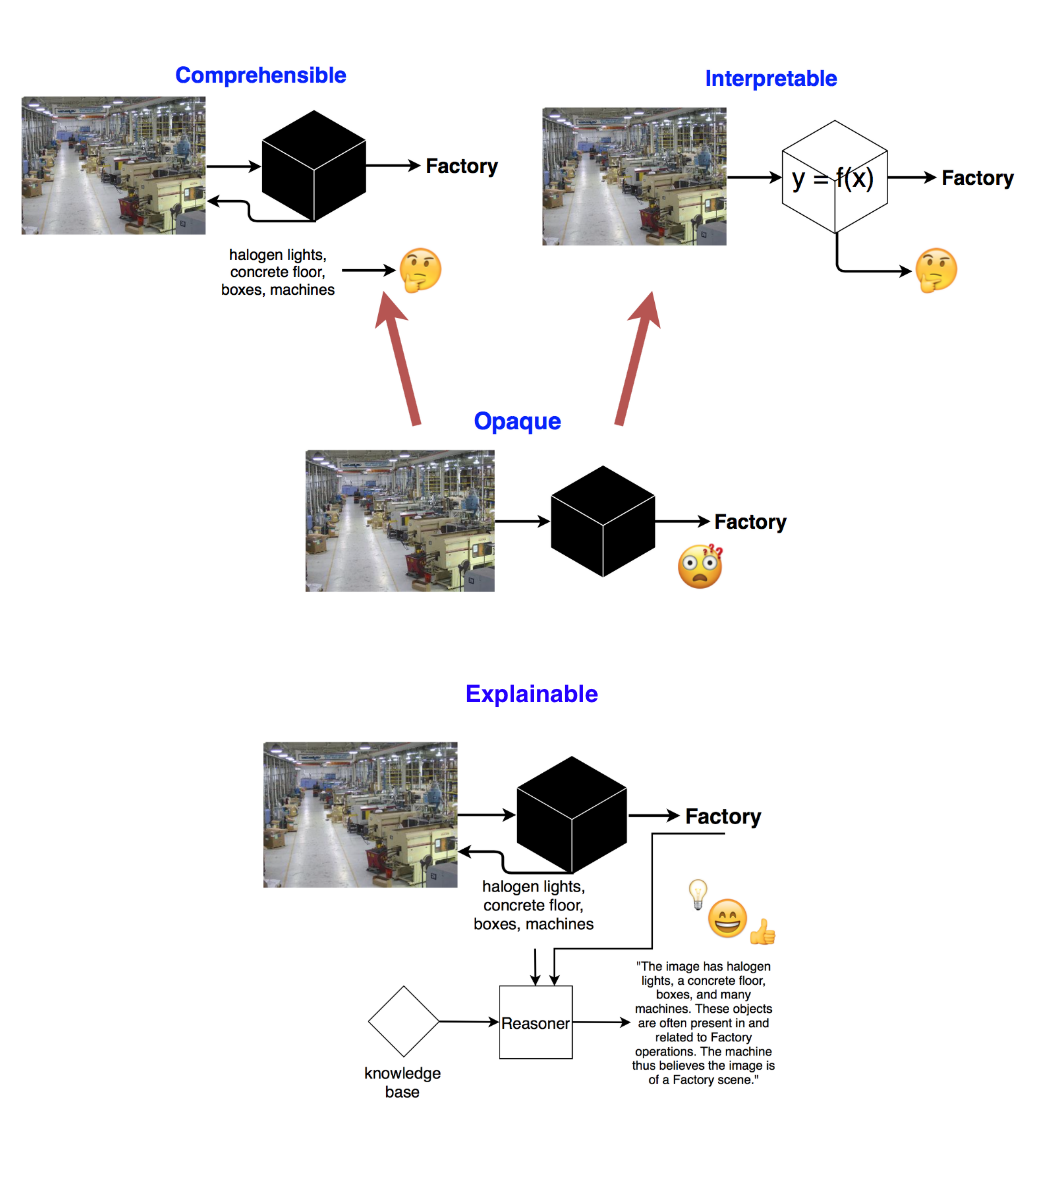
\includegraphics[width=0.9\textwidth]{introduction/images/xai-systems-taxonomy}}
\caption{The relationship between \textit{opaque}, \textit{interpretable},  \textit{comprehensible} and \textit{interpretable} systems [adapted from \citet{Doran2018}]}
\label{fig:xai-systems-taxonomy}
\end{figure}

What I hope can be gleamed from this brief introduction to the field of Explainable Artificial Intelligence, is that many of the problems it aims to tackle are hard \textit{per-se} and may not have a unique optimal solution.  
This is because these issues are not only engineering problems, but exist at the intersection between man and machine and as such can't be tackled using only the methods of Computer Science (this is what is meant by \citet{doshi2017towards} when they talk about \enquote{incompleteness in the problem formalization}).  
This is one of the main pitfalls that the xAI community finds itself falling into, as most of its researchers come from the hard-sciences domains of computer science, mathematics and statistics. 
There is little hope to define the desiderata without the guidance that can only come from philosophy, because of its millennia-long tradition in dealing with ethical issues.  
There is no way to satisfactorily move towards and evaluate these desiderata without resorting to the well-established literature and methods of the Social Sciences (for a good example of how this may work, see \citet{stumpf2009interacting}), as the human element is inherent in any explanation. 
It would be \enquote{reinventing the wheel} to try and define how a computer should relate itself to its user, when the field of Human Computer Interaction has many of these answers already. 
It should be clear that when the human - and particularly the ethical - domain are part of the equation, it is impossible \textit{by definition} to find an optimal and unique solution, that many xAI researchers seem to still regard as achievable.

Effectively, the biggest gap that can be identified is a dearth of explainability methods that have been validated not only with domain experts, but even with real humans.
Many researchers seem content with claiming \textit{formal explainability} and neglect the human half of the explanation.
An explanation, by its nature, involves and \textit{explainer}, the machine, and an \textit{explainee}, us.
Up till now, it seems that xAI is content with \enquote{explaining the explainer}, not realising that in doing so it offers no explanation at all (see \citet{mittelstadt2019explaining} for a critique of the field of xAI, based on this lack of awareness).